\mysection{Loss}
\vspace{.5\baselineskip}
    \centering
    Directly optimise Intersection-over-Union (IoU) and guide attention mechanisms.
%\begin{equation*}
%\loss[\mathrm{HART}]{\cdot} = \lambda_{\mathrm{t}} \loss[\mathrm{t}]{\cdot} + \lambda_{\mathrm{s}} \loss[\mathrm{s}]{\cdot} + \lambda_{\mathrm{a}} \loss[\mathrm{a}]{\cdot}  + \reg{ \B{\lambda} } + \beta \reg{ \cdot }
%\end{equation*}
\begin{equation*}
\loss[\mathrm{HART}]{\cdot} = \lambda_{\mathrm{t}} \loss[\mathrm{t}]{\cdot} + \lambda_{\mathrm{s}} \loss[\mathrm{s}]{\cdot} + \lambda_{\mathrm{a}} \loss[\mathrm{a}]{\cdot} + \beta \reg{ \cdot }
\end{equation*}

\begin{description}[leftmargin=\parindent,labelsep=1em]

\item[Tracking:] Negative log of Intersection-over-Union.
\begin{equation*}
    \loss[\mathrm{t}]{\data, \theta} = \expc[\p{\widehat{\bb}_{1:T}}{\bxTs, \bb_1}]{ -\log \mathrm{IoU} \fences{\widehat{\bb}_t, \bbt}}
\end{equation*}

\item[Spatial Attention:] It follows the object, but shouldn't be too big.
\begin{equation*}
    \loss[\mathrm{s}]{\data, \theta} = \expc[\p{\baTs}{\bxTs, \bb_1}]{ -\log \fences*{\frac{ \bat \cap \bbt }{\mathrm{area}\fences{\bbt}} } -\log \fences { 1 - \mathrm{IoU} \fences{\bat, \bxt} } }
\end{equation*}

\item[Appearance Attention:] Cross-entropy with dynamically created target mask $\tau \fences { \bat, \bbt }$:
$\loss[\mathrm{a}]{\data, \theta} =   \expc[\p{\baTs, \bsTs}{\bxTs, \bb_1}]{ H \fences{ \tau \fences { \bat, \bbt }, \bst  } }$.



\begin{minipage}[c]{.3\textwidth}
    \centering
    \vspace{0.75em}
    \caption*{\large With Appearance Attention Loss: Successful Tracking}
    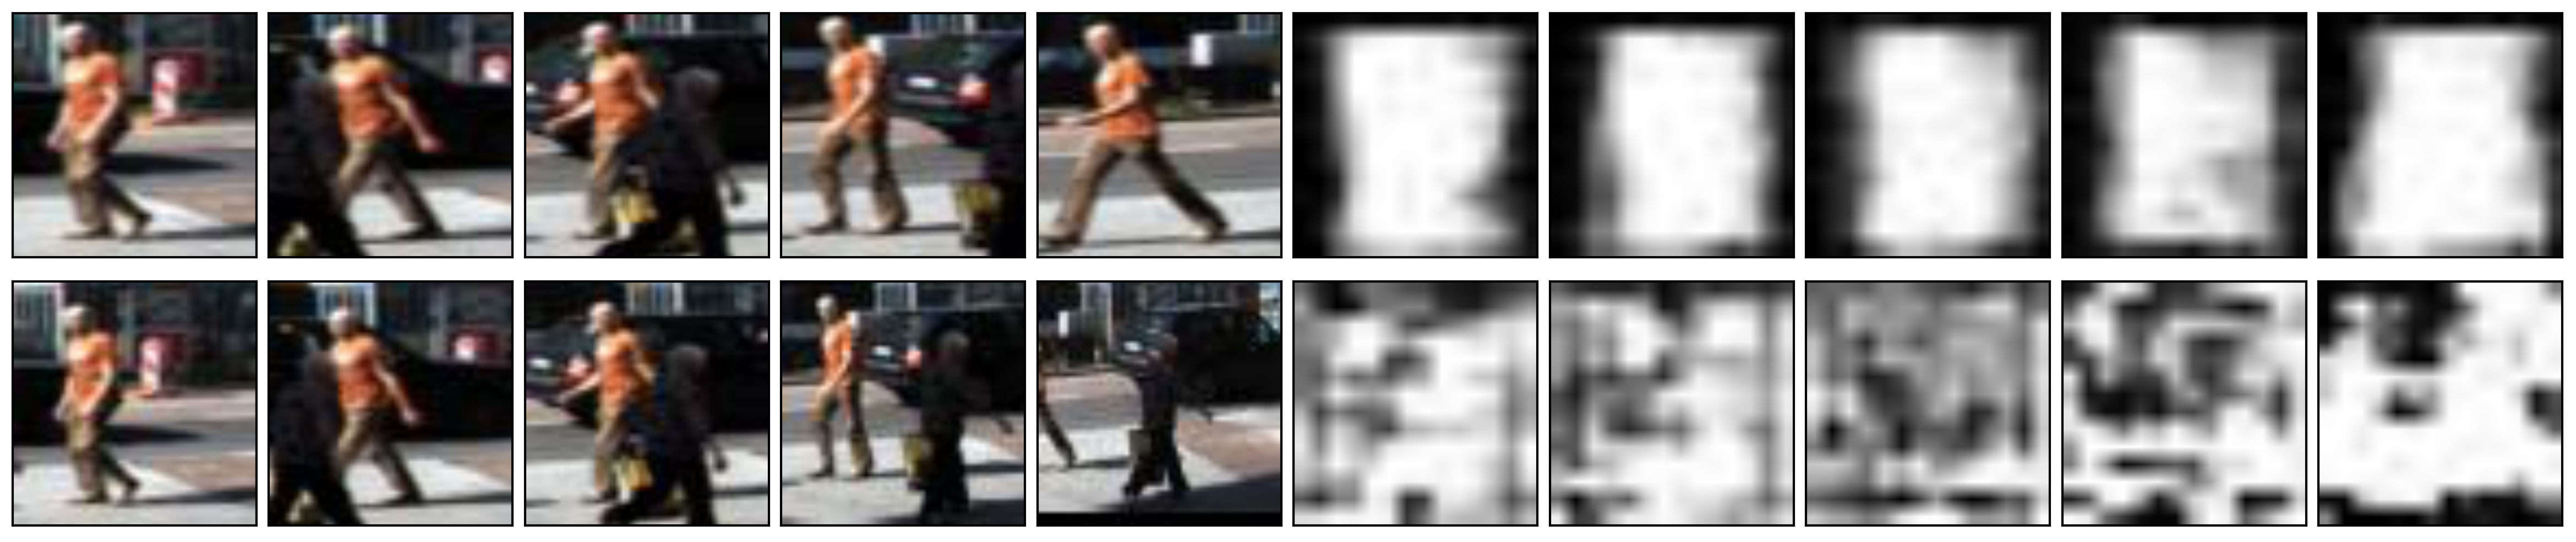
\includegraphics[width=\textwidth]{soft_id_swap}
    \caption*{\large Without Appearance Attention Loss: ID Swap}
\end{minipage}
\end{description}

